% !TEX root = ../main.tex

\begin{savequote}[99mm]
Some people would claim that things like love, joy and beauty belong to a different category from science and can't be described in scientific terms, but I think they can now be explained by the theory of evolution.
\qauthor{Stephen Hawking}
\end{savequote}

\chapter{Evolutionary solution to the identification problem}
\label{chap:id-bin}

In this chapter we describe the solution of the identification problem, for which an evolutionary algorithm based on a GA~\cite{holland1975adaptation} will be used. GAs constitute a  well-known optimization method used in many domains of application, including earlier research on CAs. For example,
GAs have been used in the construction of CA-based random number generators~\cite{TOMASSINI2001151}, for finding CAs capable of image reconstruction~\cite{Seredynski2012} and for retrieving CA-based population models of competing individuals~\cite{Schimit2014}.

For the sake of reproducibility, we formally define the GA by clearly giving the individuals' representation, structure of the population, a fitness function, the genetic operators, namely the selection procedure for reproduction, and the cross-over and mutation operators, and finally the halting conditions.

\section{Individuals and populations}
Here, the individuals that make up the population are CAs, encoded through the LUT of their local rule, which is possible since the LUT of any CA $A\in\mathcal{A}_r$ can be represented as a bit-string of length $2^{2\,r+1}$ (see Section~\ref{sec:prem}).

The population is a collection of local rules with different radii between $r_{\ast}$ and~$r^{\ast}$, since the radius of the desired solution might not be known in practice and one of the goals is to detect it. Note that as a consequence of Fact~\ref{fac:incl}, we might opt to consider populations of local rules with radius $r^{\ast}$ only, but by allowing diverse radii, populations can evolve quicker and produce simpler solutions, \emph{i.e.}\ local rules with smaller radii.

The number of CAs in a population is denoted by $P>0$. The symbol $\mathcal{P}^n$, where $n=1,2,\dotsc$, denotes the population of the $n$-th generation of the GA. Population $\mathcal{P}^1$ is the initial population, and is constructed by randomly selecting $P$ bit-strings. Let $\mathcal{P}^1 = \{L^1_1,\dotsc,L^1_P\}$, where $L^1_i$ is the $i$-th individual in the initial population, then $\abs{L^1_i} = 2^{2\,r_i+1}$ for some $r_i\in\{r_{\ast},\dotsc,r^{\ast}\}$. This radius $r_i$ can change as the GA evolves. Populations $\mathcal{P}^n$ for $n>1$ are evolved by applying the genetic operators described in the remainder of this section. Individuals belonging to the $n$-th population are denoted by $L^n_i$, for $i=1,\dotsc,P$.

\section{Fitness function}\label{sec:fitness}
The fitness function is directly related to the error measure $\widetilde{E}_{\mathcal{I}}$ defined by~\eqref{eq:error}.
% Although Proposition~\ref{fac:relationoferror} states that the error measures given by~\eqref{eq:error0} and~\eqref{eq:error} can be used interchangeably, preliminary experiments showed that the latter results in an efficient and convergent algorithm, while suboptimal results were obtained using the measure given by~\eqref{eq:error0}. This follows from the fact that the error in row $n$ is affected by errors appearing in rows $2,\dotsc,n-1$. As we know from the research on dynamical properties of CAs that small initial perturbations can strongly affect further system states\cite{jan.lyap}, it is easier to optimize $\widetilde{E}_{\mathcal{I}}$ with a GA than $E_{\mathcal{I}}$. 
Let $L\in\{0,1\}^{2^{2\,r+1}}$ be the LUT of some local rule that defines a CA $A$. Then $\fit_{\mathcal{I}}(L)$ denotes the fitness of $A$, and is defined as:
\begin{equation}
	\fit_{\mathcal{I}}(L) = C(\mathcal{I}) - M_\mathcal{I} - \widetilde{E}_\mathcal{I}(A)\,.
	\label{eq:fit-org}
\end{equation}
The fitness function takes integer values from 0 up to $C(\mathcal{I}) - M_\mathcal{I}$ which is the total number of completely observed states excluding the states in all of the initial configurations. Therefore, there are only finitely many values of the fitness function. The goal of the GA is to maximize fitness, and a CA leading to maximal fitness is a solution of the identification problem.
From the above, it is relatively clear that if $C(\mathcal{I}) - M_\mathcal{I}$ (the number of completely observed cells not counting the first rows) is close to zero then the problem is not very interesting. 
Additionally, if $C(\mathcal{I}) = M_\mathcal{I}$, then the problem is trivial because every CA is a solution.

Initial experiments have shown that the fitness function defined by~\eqref{eq:fit-org} is effective. Yet, the computing time for finding its values is unacceptable when large observation sets are considered, since the cost of computing an exact value is linear in the size of the observation set. An approximation algorithm is used to overcome this issue for a large observation set. During the evolution of the $n$-th population, we estimate the value of $\fit_{\mathcal{I}}$ by using $\fit_{\mathcal{I}_n}$, where $\mathcal{I}_n\subset\mathcal{I}$ is a non-empty subset. Such an approach is justified by Fact~\ref{fac:rules-set}, which assures that the solution set is not being reduced. The set $\mathcal{I}_1$ is a subset of $0<s\leq \abs{\mathcal{I}}$ randomly selected observations of $\mathcal{I}$, while the set $\mathcal{I}_{n+1}$, for $n\geq 1$, is built from $\mathcal{I}_{n}$ by replacing one of its observations denoted by $I_r$, with a new selection from $\mathcal{I} \backslash \mathcal{I}_{n}$ denoted by $I_a$. There are two scenarios for selecting~$I_r$ and~$I_a$, depending on the contents of $\mathcal{I}_n$, which are presented below.

Let $B(n)$ yield the fittest individual from the $n$-th population, {\it i.e.}\
\begin{equation}
	B(n) = \argmax_{L\in\mathcal{P}^{n}} \fit_{\mathcal{I}_{n}}(L)\,.
\end{equation}
If multiple choices of $B(n)$ are possible, we pick one at random.
As described in more detail in Section~\ref{sec:halt}, for such an individual, the fitness $\fit_{\mathcal{I}}$ over the entire set $\mathcal{I}$ is recalculated verifying  whether the halting condition is satisfied at every iteration of the GA. Consequently, we have access to the values $\widetilde{E}_I(B(n))$ for any $I\in\mathcal{I}$, and thus we can easily find $I^{\ast}\in\mathcal{I}$ such that $\widetilde{E}_{I^{\ast}}(B(n)) \geq \widetilde{E}_I(B(n))$ for any $I\in\mathcal{I}$.

If $I^{\ast} \in \mathcal{I}_{n}$, then $I_r$ is selected randomly from $\mathcal{I}_{n}$ in such a way that $I_r \neq I^{\ast}$ and $I_a$ is also selected randomly from $\mathcal{I}\backslash \mathcal{I}_{n}$. On the other hand, if $I^{\ast} \not\in \mathcal{I}_{n}$, then $I_a = I^{\ast}$ and~$I_r$ is selected randomly from $\mathcal{I}_{n}$. Formally, the goal of this procedure is to assure that the observation resulting in the highest error $I^{\ast}$ is included in $\mathcal{I}_{n+1}$ and that exactly one observation is replaced at every generation, \emph{i.e.}\ $\abs{\mathcal{I}_{n} \cap \mathcal{I}_{n+1}} = s-1$.
In Algorithm~\ref{algo:ga}, we use $\Fbuildset{$\mathcal{I}_n, E^n$}$ to denote the subset $\mathcal{I}_{n+1}$ obtained according to the procedure outlined above. The argument $E^n$ corresponds to the error vector of the individual $B(n)$, \emph{i.e.}\ $E^n = \big(\widetilde{E}_I(B(n))\big)_{I\in\mathcal{I}}$. Further, $\Ferrorvec{$L, \mathcal{I}$}$ denotes a function that returns a vector of the form $(\widetilde{E}_{I}(L))_{I\in\mathcal{I}}$.

Let $F(n)$ denote the highest fitness observed among the individuals that had the highest values of fitness estimation during the GA evolution up to the $n$-th generation. Let $n\in\mathbb{N}$, then $F(n)$ is defined as $F(n) = \max_{i\in\{1,\dotsc,n\}} \fit_{\mathcal{I}}\left(B(i)\right)$.

Obviously $F(n)\leq F(n+1)$. In addition to this maximal fitness $F$, we also define the age of this value as the number of GA iterations during which the maximal fitness did not change. Formally, a value $F(n)$ has an age $a(n)>0$ if and only if it holds that:
\[F(n-a(n)-1) < F(n-a(n)) = \cdots = F(n-1) = F(n)\,.\]

\section{Selection}\label{sec:select}
% Here we define the selection operator. It is used for selecting the parent individuals for reproduction. 
We use a standard, random selection method. The probability of selecting a given individual is proportional to its fitness. This is feasible, since the fitness function introduced in Section~\ref{sec:fitness} is bounded. The selection process is repeated with replacement, so that each of the individuals can be selected multiple times.
In the pseudo-code, the function $\selectParents{$\mathcal{P}$}$ returns two individuals selected from population $\mathcal{P}$ according to this selection procedure.

\section{LUT rescaling}\label{sec:rescal}
Before describing the cross-over operator, we introduce a rescaling operation in order to be able to define cross-over of LUTs with different radii. Given Fact~\ref{fac:incl}, each CA defined by a local rule with neighborhood radius $r$, can also be defined by a local rule with neighborhood radius $r+1$. A simple method for ``converting'' the LUT of a given local rule $f$, with radius $r$, to the LUT of its corresponding local rule $f^\uparrow$, with radius $r+1$, follows from the fact $f^\uparrow(s_1, \dotsc, s_{2\,(r+1)+1}) = f(s_2,\dotsc,s_{2\,r+2})$, for all $s_1,\dotsc,s_{2\,(r+1)+1}\in\{0,1\}$. Note that both $f$ and $f^\uparrow$ define the same CA. The operation of increasing the radius by one will be referred to as up-scaling by one. Let $L\in\{0,1\}^{2^{2\,r+1}}$ be the LUT of $f$, then the LUT of $f^\uparrow$, denoted as $L^\uparrow\in\{0,1\}^{2^{2(r+1)+1}}$, can be constructed from $L$ using Algorithm~\ref{algo:up}.

\begin{figure}[!t]
	\removelatexerror\begin{algorithm}[H]
		\KwIn{LUT given by variable $L$.}
		\KwOut{Up-scaled LUT stored in variable $L^\uparrow$.}
		\For{$i=1,\dotsc,2^{2\,r+1}$}{
		$L^\uparrow[2\,i] \gets L[i]$\;
		$L^\uparrow[2\,i-1] \gets L[i]$\;
		$L^\uparrow[2\,i-1+2^{2\,r+2}] \gets L[i]$\;
		$L^\uparrow[2\,i+2^{2\,r+2}] \gets L[i]$\;
		}
		\caption{Up-scaling of the LUT}\label{algo:up}
	\end{algorithm}
\end{figure}

Similarly to the up-scaling operation, we define the inverse operation. Let $f$ be a local rule with neighborhood radius $r$, then the down-scaled local rule $f_\downarrow$, with radius $r-1$, is defined as:
\begin{equation*}
	f_\downarrow(s_1,\dotsc,s_{2\,r-1}) = \left[\frac{1}{4}\sum_{a=0}^{1}\sum_{b=0}^{1}f(a,s_1,\dotsc,s_{2\,r-1},b)\right],
\end{equation*}
where $[\cdot]$ indicates rounding to the nearest integer (we assume $[0.5]=0$). The method of computing the LUT of the down-scaled rule is presented in Algorithm~\ref{algo:down}. Let $L\in\{0,1\}^{2^{2\,r+1}}$ be the LUT of some local rule $f$, then this algorithm constructs the LUT $L_\downarrow\in\{0,1\}^{2^{2\,r-1}}$ corresponding to the local rule $f_\downarrow$. It is easy to see that, in general, $f$ and $f_\downarrow$ define different CAs. Informally, $f_\downarrow$ should be understood as the closest approximation of $f$ with a smaller radius.

\begin{figure}[!t]
	\removelatexerror\begin{algorithm}[H]
		\KwIn{LUT given by variable $L$.}
		\KwOut{Down-scaled LUT stored in variable $L_\downarrow$.}
		Initialize $C[i]\gets 0$ for $i=1,\dotsc,2^{2\,r-1}$\;
		\For{$i=0,\dotsc,2^{2\,r+1}-1$}{
		$j\gets 1 + (i/2\ \text{mod}\ 2^{2\,r-1})$\;
		$C[j] \gets C[j] + L[i+1]$\;
		}
		\For{$i=1,\dotsc,2^{2\,r-1}$}{
		\If{$C[i]>2$}{
			$L_\downarrow[i] \gets 1$}
		\Else{$L_\downarrow[i]\gets 0$}
		}
		\caption{Down-scaling of the LUT}\label{algo:down}
	\end{algorithm}
\end{figure}

Using the up-scaling and down-scaling operations, we can define a general rescaling operation from radius $r$ to $r'$, by applying up-scaling (when $r'>r$) or down-scaling (when $r'<r$) operations multiple times.
The function rescaling a LUT $L$ from radius $r$ to radius $r'$ will be denoted as $\scaleToRadius{$L,r'$}$ in the pseudo--code. This function returns $L$ if $r'=r$. 

\section{Cross-over}
To produce offspring, two parents are selected according to the selection  procedure outlined in Section~\ref{sec:select}. If the radii of the selected parents are equal, we use uniform cross-over, \emph{i.e.}\ the result is a vector $L_c$ with values that are randomly selected from the parents $L_1$ and $L_2$ so that $\mathbb{P}(L_c[i] = L_1[i]) = \mathbb{P}(L_c[i] = L_2[i]) = 0.5$. If $r_1\neq r_2$, then the LUTs are rescaled before applying crossover. Assuming that $r_1 < r_2$, the radius $r$ of the resulting rule is selected randomly from the set $\{r_1, r_{1}+1, \dotsc, r_2\}$, after which the parents are rescaled to the radius $r$ and the cross-over operator is applied.

In Algorithm~\ref{algo:cross} the pseudo-code summarizing the crossover operation is given. The function $\rand{}$ returns pseudo--random numbers from the interval $[0,1]$ with a uniform distribution, $\randInt{a,b}$ returns a randomly selected integer $n\in\{a,a+1,\dotsc,b\}$, while the function $\radius{L}$ returns the radius of the local rule defined by the LUT $L$. Its value is equal to $(\log_2(\abs{L})-1)/2$, where $\abs{L}$ is the length of the vector $L$. 

\begin{figure}
\removelatexerror
\begin{algorithm}[H]
\KwIn{LUTs $L_1$, $L_2$ to be crossed.}
\KwOut{Result of the cross-over operator.}
\Fn{\cross{$L_1, L_2$}}{
$r_1 \gets \fmin{\radius{$L_1$}, \radius{$L_2$}}$\;
$r_2 \gets \fmax{\radius{$L_1$}, \radius{$L_2$}}$\;
$r\gets \randInt{$r_1$, $r_2$}$\;
$L_1\gets \scaleToRadius{$L_1$, $r$}$\;
$L_2\gets \scaleToRadius{$L_2$, $r$}$\;
$L\gets L_1$\;
\For{$i=1,\dotsc,2^{2\,r+1}$}{
\If{$\rand{} < 0.5$}{
$L[i]\gets L_2[i]$\;
}
}
\Return{L}\;
}
\caption{Cross-over operation}
\label{algo:cross}
\end{algorithm}
\end{figure}

\section{Mutation operator}
Finally, the offspring individuals are mutated. Here, three types of mutations are used: bit flipping, decrease of radius and increase of radius. The latter two mutations simply rely on the down-scaling or up-scaling operations outlined in Algorithms~\ref{algo:up} and~\ref{algo:down}, and introduce diversity in the length of the individuals, while bit flipping randomly flips selected bits in the LUT of the individual.

Mutations are applied in a well-defined order. Firstly, with probability $p_u$, up-scaling is applied. After that, we flip randomly selected bits. The bit-flip mutation is applied bit-by-bit independently. The probability $p_f$ of mutating a bit is defined as follows:
\begin{equation}
	p_f(n) = e^{-\alpha \, (R - a(n))}\,,
\end{equation}
for some $\alpha>0$ and $R\in\mathbb{N}$. The role of the parameter $R$ is described in more detail in Section~\ref{sec:elite}. For now, we may assume that $a(n)$ will never be higher than $R$ and thus, $p_f(n) \leq 1$. This formula is motivated by the fact that when the age $a(n)$ is low, the probability of mutation should also be relatively low in order to give the algorithm a chance to fine-tune the solution. If this fine-tuning fails, the age $a(n)$ increases and the population tends to freeze near a local optimum. In order to escape from it, we then apply mutation with a higher probability. Such a procedure is partially effective due to the elite survival procedure introduced in Section~\ref{sec:elite}. Finally, after applying bit-flipping, we apply down-scaling with probability $p_d$.

This order of application is chosen because the number of possibilities to be affected by bit-flipping increases by first applying up-scaling. Besides, performing the down-scaling at the end of the sequence of mutation operators allows to evolve simpler rules.
Algorithm~\ref{algo:mutate} gives the pseudo-code describing the mutation operator. 

\begin{figure}
\removelatexerror
\begin{algorithm}[H]
\KwIn{LUT and the age of the best individual.}
\KwOut{LUT of the mutant.}
\Fn{\mutate{$L,age$}}{
$r\gets \radius{L}$\;
\If{$\rand{} < p_u$}{
$L\gets \scaleToRadius{$L, r+1$}$\;
$r\gets r+1$\;
}
\For{$i\gets 1,\dotsc,2^{2\,r+1}$}{
\If{$\rand{} < e^{-\alpha \, (R - age)}$}{
$L[i]\gets 1-L[i]$\;}
}
\If{$\rand{} < p_d$}{
$L\gets \scaleToRadius{$L, r-1$}$\;
}

\Return{L}\;
}
\caption{Mutation operation}
\label{algo:mutate}
\end{algorithm}
\end{figure}

\section{Elite survival and population re-initiation}\label{sec:elite}
After evolving a new population, an elite survival procedure is applied, which has shown to be a pre-requisite to reach convergence. The procedure is implemented by selecting the $P_E \ll P$ fittest individuals from the previous population and letting them replace randomly selected individuals in the newly evolved one.
In the pseudo-code \Fcopyelite{$\mathcal{P}_{\textrm{\upshape new}}, \mathcal{P}_{\textrm{\upshape old}}, F_{\textrm{\upshape old}}$} denotes the procedure that copies the $P_E$ fittest individuals from population $\mathcal{P}_{\textrm{old}}$ to $\mathcal{P}_{\textrm{new}}$. The third argument $F_{\textrm{old}}$ denotes the vector of fitness values of individuals in population~$\mathcal{P}_{\textrm{old}}$.

Including this elite survival procedure dramatically increases the performance of the algorithm, though there are cases where such an approach causes the population to progress towards a local optimum. Our experiments showed that the best way to overcome this is to apply a re-initiation procedure. If for a given $n$ it holds that the age $a(n) = R$, then we re-initiate the algorithm by replacing the current population with a new, randomly selected set of CAs. In other words, we do not allow a situation where the age of the best individual evolved so far is higher than $R$. Such an approach might seem to contradict the evolutionary nature of the algorithm, but the use of a dynamic mutation probability $p_f(n)$ and an elitist survival procedure relates it to the evolution of multiple separated genetic islands~\cite{Whitley98theisland}, out of which the one with the fittest individual is selected after a predefined number of iterations.

\section{Halting conditions}\label{sec:halt}
The GA evolves until a CA that fits the observation set is discovered or a predefined number of GA iterations passes.
%   In practice, we have to impose a limit on the maximal allowable number of GA iterations, as such ensuring that the computation finishes in finite time. 

As mentioned in Section~\ref{sec:fitness}, the fitness $\fit_{\mathcal{I}}$ is approximated by $\fit_{\mathcal{I}'}$ for some $\mathcal{I}'\subset\mathcal{I}$, which is effective for selection, but cannot be used to verify whether the halting condition has been met.
%  since $\fit_{\mathcal{I}'}(A) = C(\mathcal{I}') - M_\mathcal{I}'$ for some CA $A$ does not imply $\fit_{\mathcal{I}}(A) = C(\mathcal{I}) - M_\mathcal{I}$. 
Therefore, for the individual $A$ with the highest value of $\fit_{\mathcal{I}'}(A)$, we also calculate $\fit_{\mathcal{I}}(A)$.
%  and verify whether the halting condition is met for this value, \emph{i.e.}\ 
The algorithm stops as a CA $A$ is found such that $\widetilde{E}_\mathcal{I}(A) = 0$. The knowledge of $\fit_\mathcal{I}(A)$ at every iteration is exploited to build subsets $\mathcal{I}_n\subset\mathcal{I}$ used for estimating $\fit_\mathcal{I}$ (see Section~\ref{sec:fitness}).

\section{Outline of the algorithm}
As a summary of the description we present the pseudo-code of the GA algorithm in Algorithm~\ref{algo:ga}. In the pseudo-code, $\calculateFitness{$\mathcal{P}, \mathcal{I}_n$}$ denotes a function returning a vector $(\fit_{\mathcal{I}_n}(L))_{L\in\mathcal{P}}$. Additionally, the function: 
\[\Fbest{$(\fit_{\mathcal{I}_n}(L))_{L\in\mathcal{P}^n}, \mathcal{P}^n, F(n-1), a(n-1)$}\,,\] 
returns a tuple $(F(n), B(n), a(n))$.

\begin{figure}
\removelatexerror
\begin{algorithm}[H]
\KwIn{Set of observations $\mathcal{I}$.}
\KwOut{Solution stored in $best$.}
Initialize population $\mathcal{P}^1$ with randomly selected LUTs\;
Initialize $\mathcal{I}_1\subset \mathcal{I}$ with $s$ randomly selected elements\;
$\Phi^{1} \gets \calculateFitness(\mathcal{P}^{1}, \mathcal{I}_1)$\;
$mF, best, age \gets \Fbest{$\Phi^{1}$, $P^{1}$, 0, 0}$\;
$E^{1} \gets \Ferrorvec{best, $\mathcal{I}$}$\;
$n\gets 1$\;
\While{$\Fsum{$E^n$} > 0$}{

\If{age = R}{
Initialize population $\mathcal{P}^n$ with randomly selected LUTs\;
}
\Else{
\For{$i\gets 1,\dotsc,P$}{
$(P_m,P_f) \gets \selectParents{$\mathcal{P}^n$}$\;
$P_c \gets \cross{$P_m, P_f$}$\; 
$\mathcal{P}^{n+1}[i] \gets \mutate{$P_c, age$}$\;
} 
\Fcopyelite{$P^{n+1}$, $P^n$, $\Phi^n$}\;
}
$\Phi^{n+1} \gets \calculateFitness(\mathcal{P}^{n+1}, \mathcal{I}_{n})$\;
$mF, best, age \gets \Fbest{$\Phi^{n+1}$, $P^{n+1}$, mF, age}$\;
$E^{n} \gets \Ferrorvec{best, $\mathcal{I}$}$\;
$\mathcal{I}_{n+1} \gets \Fbuildset{$\mathcal{I}_n$, $E^{n}$}$\;
$n\gets n+1$\;
}
\caption{GA solving the identification problem.}\label{algo:ga}
\end{algorithm}
\end{figure}

\section{Examples: Identification of ECAs 150 and 184}\label{sec:example1}
Having described the GA for solving the identification problem, we now present an example to illustrate its behavior. An in-depth study of its performance and limitations can be found in Section~\ref{sec:experiments}.

\begin{table}[ht]
	\caption{Values of the design parameters used for the identification of ECAs 150 and 184.}\label{tab:example-params}
	\centering
	\begin{tabular}{>{$}c<{$}|>{$}c<{$}|l}
		\textrm{{\bf parameter}} & \textrm{{\bf value}} & {\bf description}                                   \\ \hline
		r_{\ast}                 & 2                    & minimal rule radius                                 \\
		r^{\ast}                 & 5                    & maximal rule radius                                 \\\hline
		P                        & 192                  & number of individuals in population                 \\
		P_E                      & 24                   & elite size                                          \\ \hline
		\Gamma                   & 10                   & upper bound for the time gaps                       \\
		S                        & 69                   & number of rows / columns in each observation        \\
		K                        & 64                   & number of observations                              \\
		s                        & 8                    & number of samples for fitness approximation         \\ \hline
		\alpha                   & 0.01                 & parameter for the dynamic mutation probability      \\
		p_d                      & 0.01                 & down-scale mutation probability                     \\
		p_u                      & 0.01                 & up-scale mutation probability                       \\ \hline
		R                        & 250                  & maximal age of fittest individual for re-initiation \\ \hline
		G                        & 9\times 10^5         & maximum number of GA iterations per run             \\
	\end{tabular}
\end{table}

For this purpose, a GA with design parameters as listed in Table~\ref{tab:example-params} was used.
These values were chosen on the basis of preliminary experiments, while the choice of $r_\ast$ was motivated by the fact that observation sets resulting from ECAs will be used. If $r_\ast=1$ would be used, the GA would be able to rapidly explore the entire space of ECAs (consisting of only 256 candidates), which makes that more interesting characteristics of the GA might be missed.

Using these parameters two experiments were conducted, further referred to as R1 and R2. In R1, the considered observation set consisted of observations of ECA 150, while ECA 184 was used in R2. The choice of these two ECAs was motivated by the fact that ECA 150 shows a strong sensitive dependence on the initial configuration, while ECA 184 (known as the traffic rule) results in an orderly behavior~\cite{citeulike:9312129}. These two types of behavior can be seen in the space-time diagrams in Figs.~\ref{fig:st-eca150} and~\ref{fig:st-eca184}. In this figure, also the corresponding temporally incomplete observations with random time gaps of at most ten time steps are shown (Figs.~\ref{fig:ob-eca150} and~\ref{fig:ob-eca184}). Such temporally incomplete observations with random time gaps, starting from 64 different initial configurations, were used by the GA.

\begin{figure*}
	\centering
	\subfloat[]{\fbox{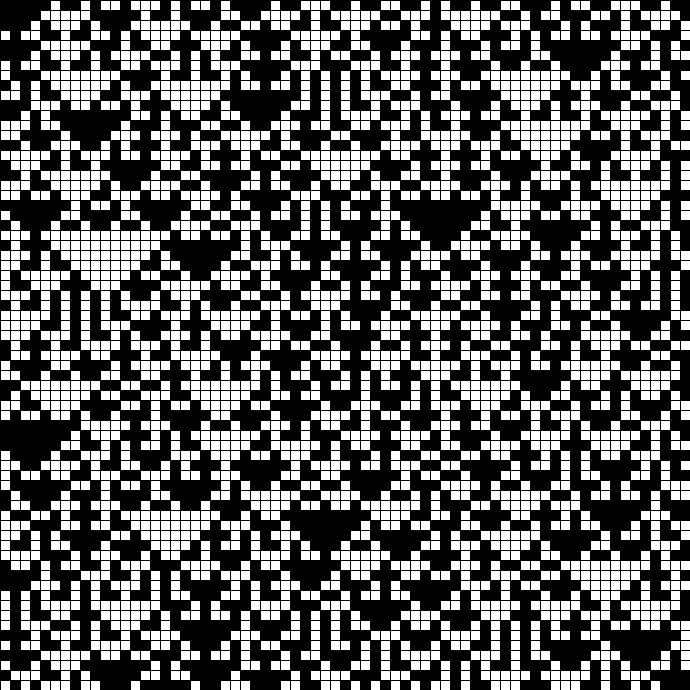
\includegraphics[width=0.33\textwidth]{figs/rule-150b.png}}\label{fig:st-eca150}}\quad
	\subfloat[]{\fbox{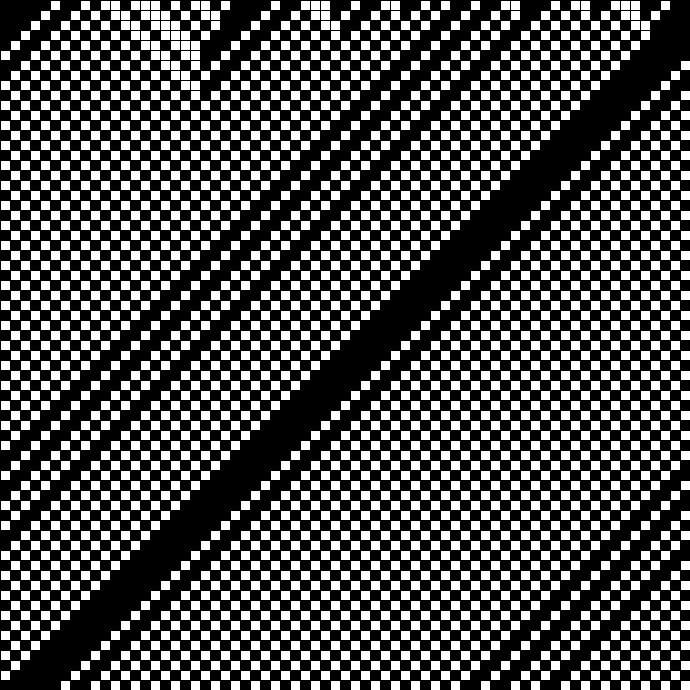
\includegraphics[width=0.33\textwidth]{figs/rule-184b.png}}\label{fig:st-eca184}}\\
	\subfloat[]{\fbox{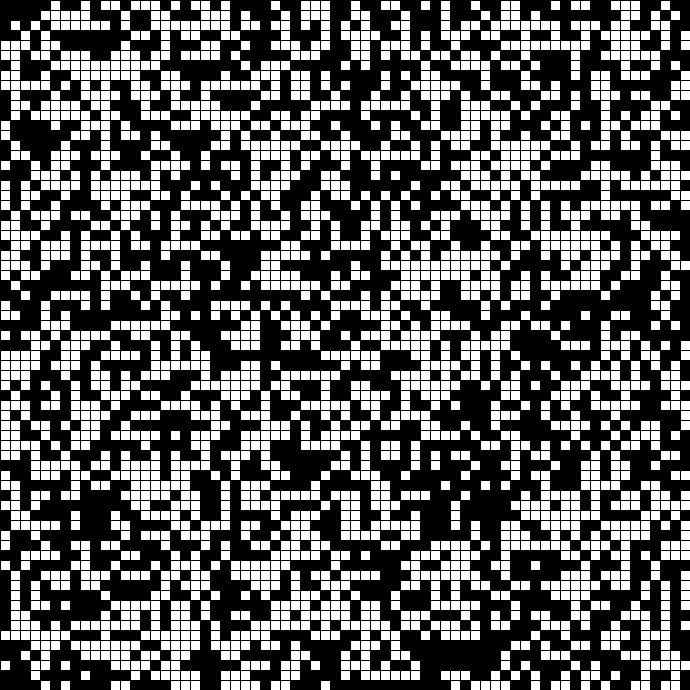
\includegraphics[width=0.33\textwidth]{figs/rule-150-gap.png}}\label{fig:ob-eca150}}\quad
	\subfloat[]{\fbox{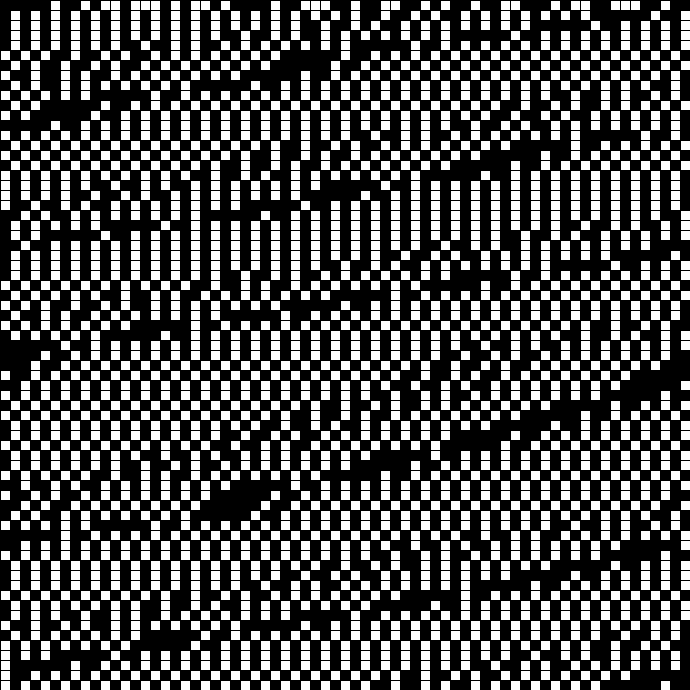
\includegraphics[width=0.33\textwidth]{figs/rule-184-gap.png}}\label{fig:ob-eca184}}
	\caption{Space-time diagrams of (\protect\subref*{fig:st-eca150}) ECA 150 and (\protect\subref*{fig:st-eca184}) ECA 184 containing 69 cells and 69 time stamps each, and the (\protect\subref*{fig:ob-eca150}), (\protect\subref*{fig:ob-eca184}) corresponding temporally incomplete observations with random time gaps of at most ten time steps.}\label{fig:space-time-example}
\end{figure*}

In both experiments, the GA quickly found a solution. In the case of experiment R1 it took 26 iterations, while 23 iterations were needed in experiment R2. In Fig.~\ref{fig:example-fitness} the maximum, average and minimum fitness of the population is shown over time for both experiments. Note that for the sake of readability the fitness values were normalized to the interval $[0,100]$.

\begin{figure}
	\centering
	\subfloat[]{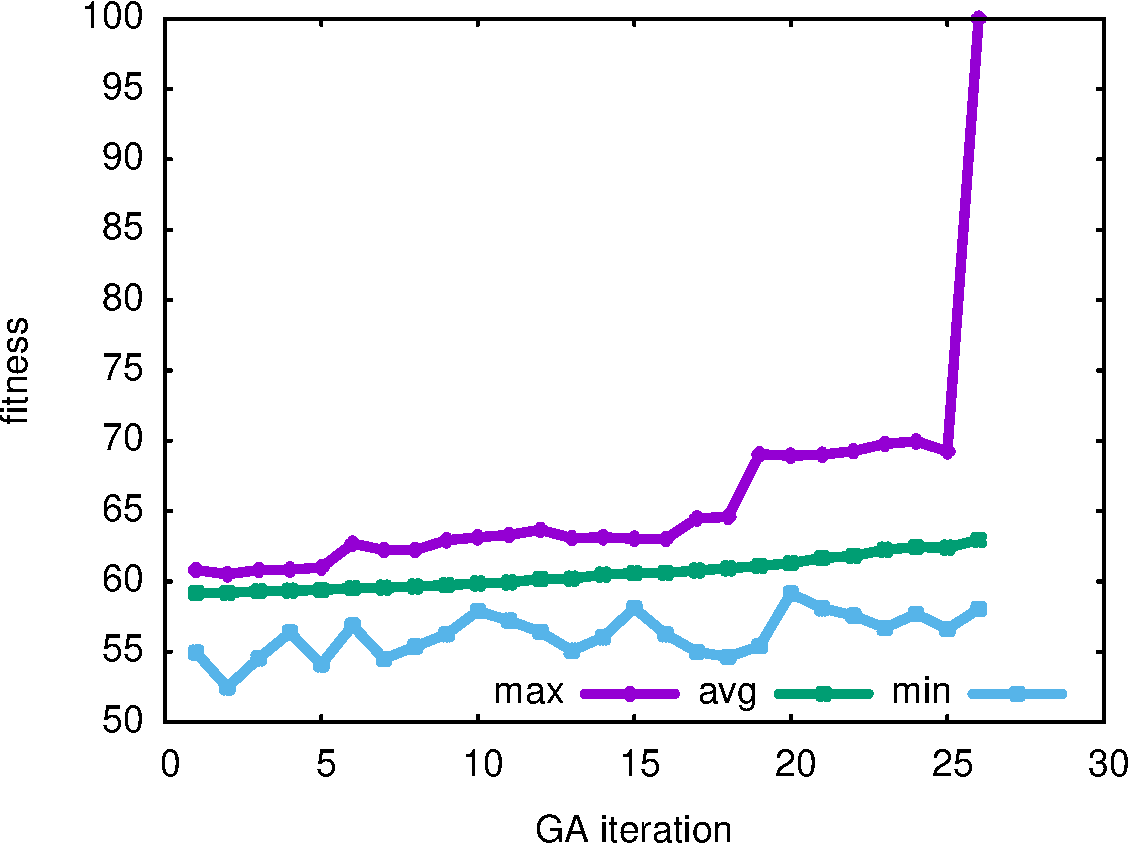
\includegraphics[width=0.45\textwidth]{figs/fit-150-crop.pdf}\label{fig:example-fit-r1}}\
	\subfloat[]{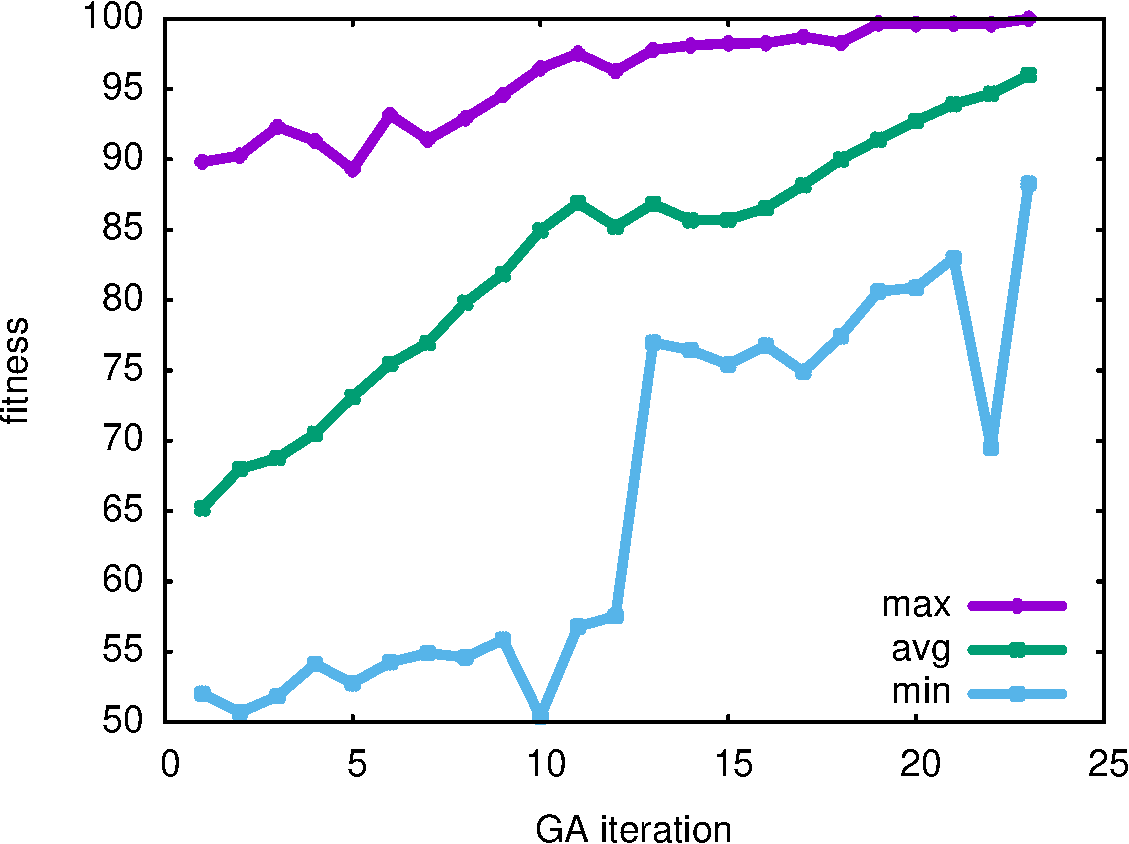
\includegraphics[width=0.45\textwidth]{figs/fit-184-crop.pdf}\label{fig:example-fit-r2}}
	\caption{The maximum, average and minimum fitness of the population versus the GA iteration in experiments (\protect\subref*{fig:example-fit-r1}) R1 and (\protect\subref*{fig:example-fit-r2}) R2.}\label{fig:example-fitness}
\end{figure}

Firstly, let us note that the plotted values correspond to the fitness approximation calculated over a subset of the observation set as described in Section~\ref{sec:fitness}. This explains why the maximum is not strictly increasing, though the algorithm uses an elite survival procedure.

Moreover, as can be seen in the plots, in both experiments the average fitness (almost) constantly increased as the populations evolved. In R1 the growth was stable but slow, while in the case of R2 we see a more rapid increase, especially during the first 10 iterations. In the case of R1, the final solution was found within one significant ``jump'' of the maximal fitness. This can be attributed to the fact that the behavior of CAs that are very close to the best solution is completely different from the one of ECA 150. In contrast, in R2 we see a rather gentle increase of the maximum fitness towards 100, which can be explained by the fact that there are many CAs resulting in checkerboard-like patterns similar to the ones evolved by ECA 184.

\begin{figure*}
	\centering
	\begin{tabular}{ccccc}
		\fbox{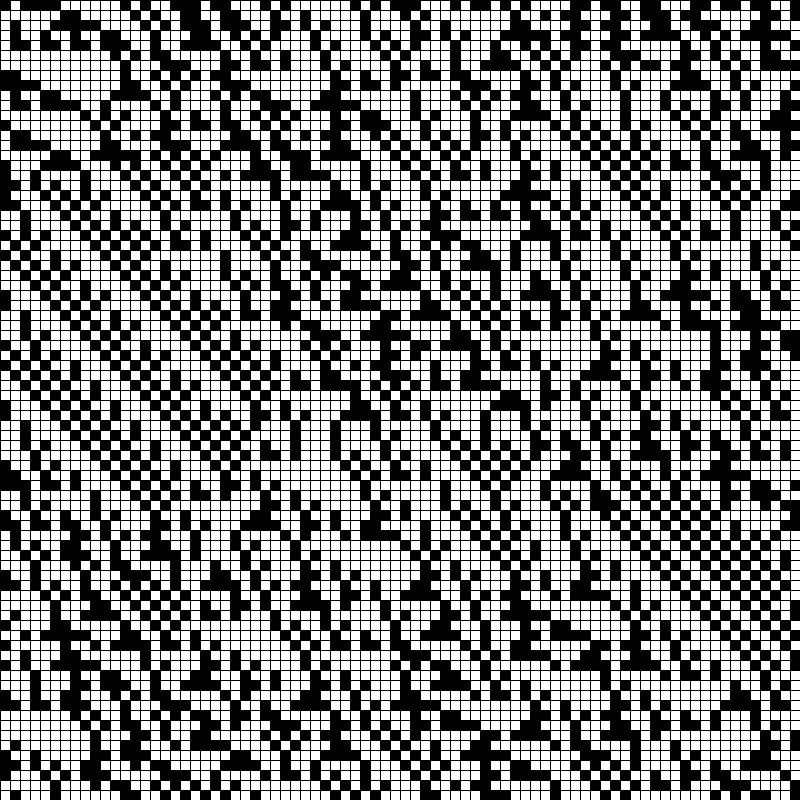
\includegraphics[width=0.17\textwidth]{figs/rule-150-best/rule-150-eval-1.png}}
		  &
		\fbox{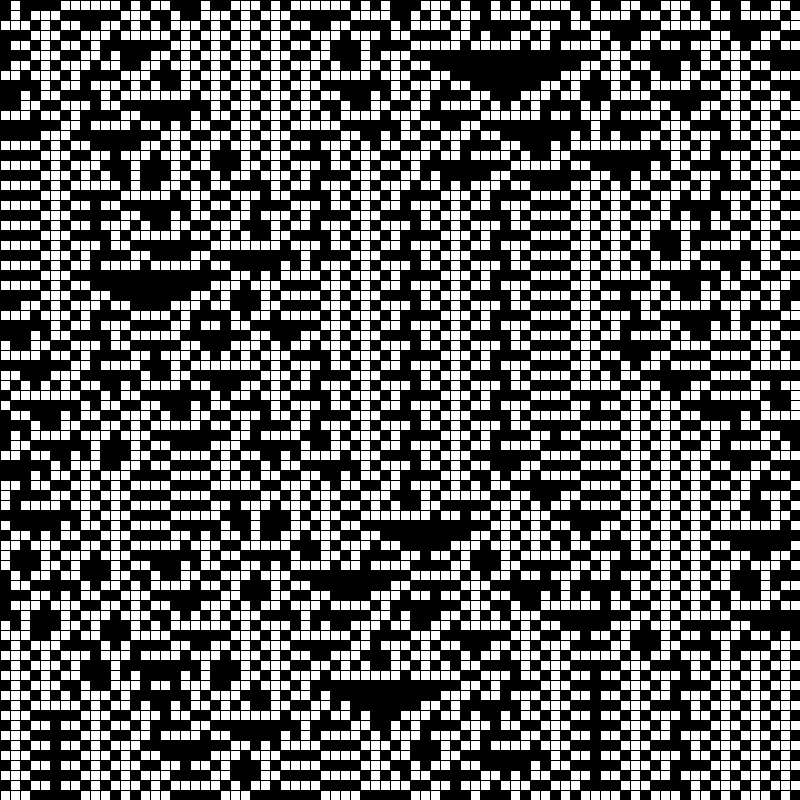
\includegraphics[width=0.17\textwidth]{figs/rule-150-best/rule-150-eval-2.png}}
		  &
		\fbox{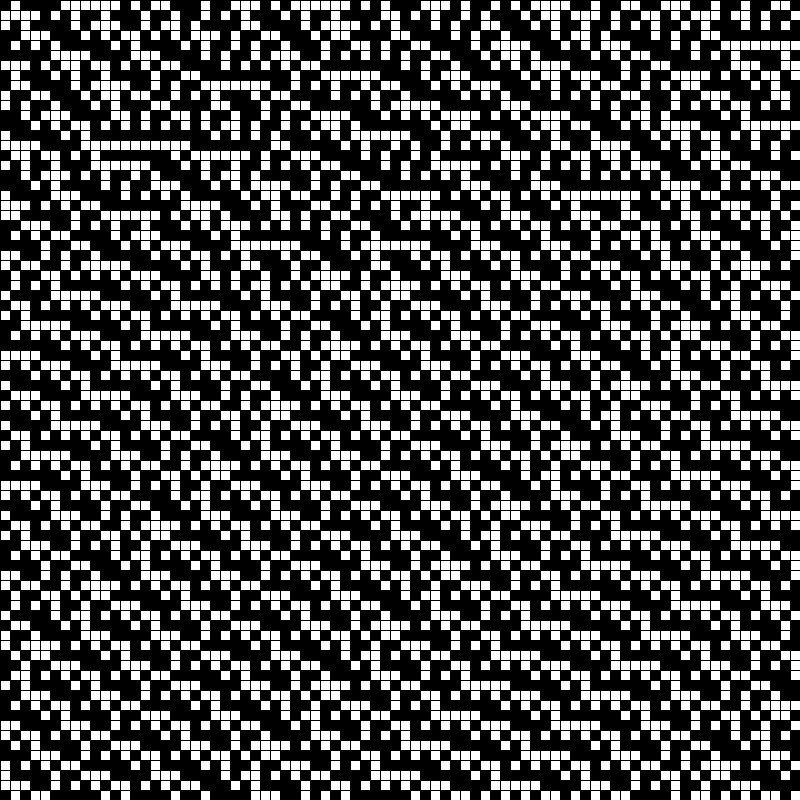
\includegraphics[width=0.17\textwidth]{figs/rule-150-best/rule-150-eval-3.png}}
		  &
		\fbox{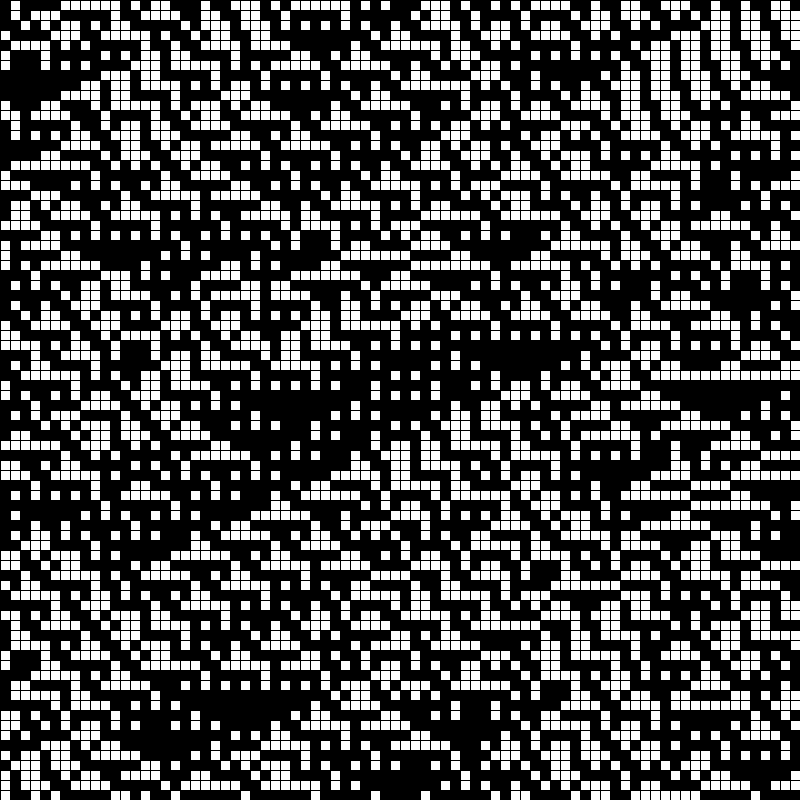
\includegraphics[width=0.17\textwidth]{figs/rule-150-best/rule-150-eval-4.png}}
		  &
		\fbox{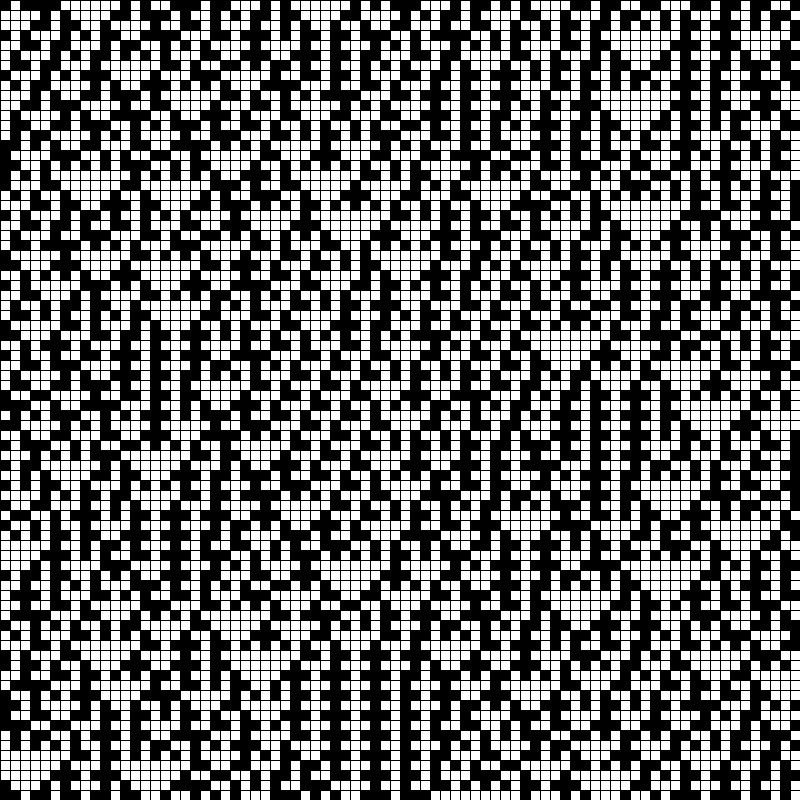
\includegraphics[width=0.17\textwidth]{figs/rule-150-best/rule-150-eval-5.png}}
		\\
		1 & 3  & 4  & 5  & 6                                                              \\
		\fbox{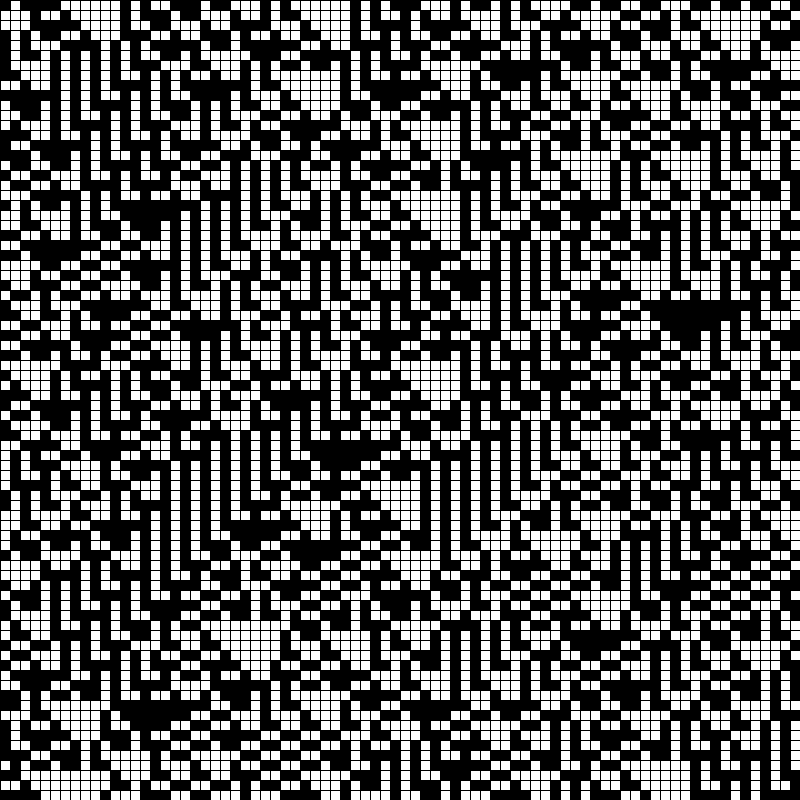
\includegraphics[width=0.17\textwidth]{figs/rule-150-best/rule-150-eval-6.png}}
		  &
		\fbox{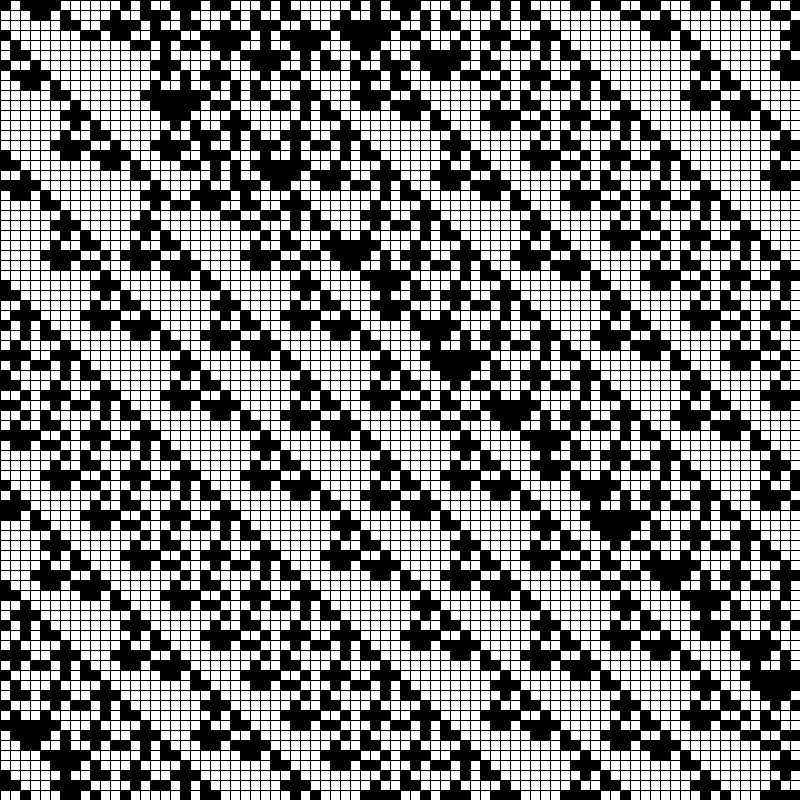
\includegraphics[width=0.17\textwidth]{figs/rule-150-best/rule-150-eval-10.png}}
		  &
		\fbox{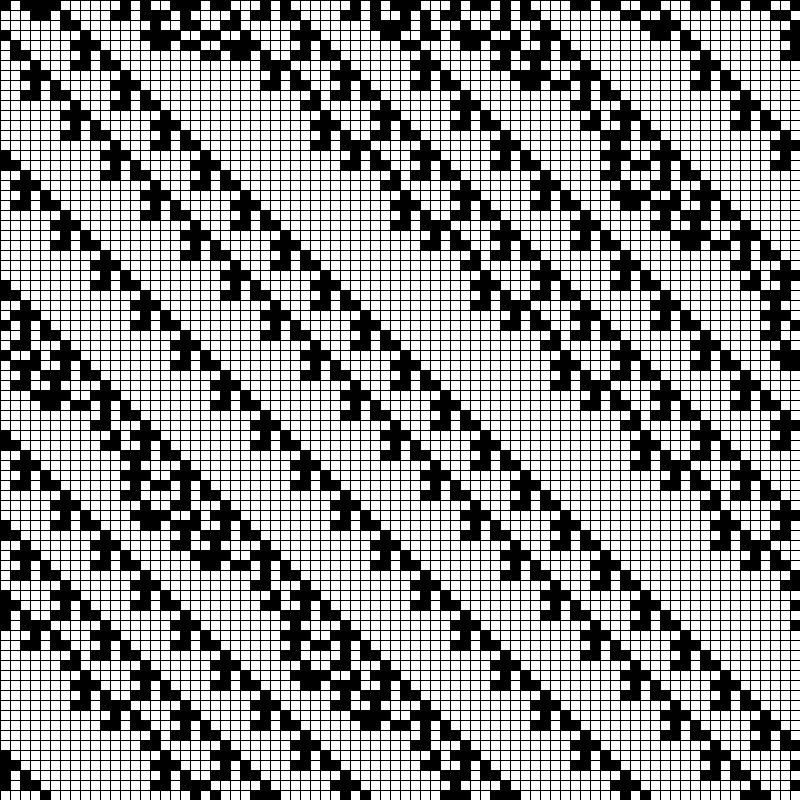
\includegraphics[width=0.17\textwidth]{figs/rule-150-best/rule-150-eval-12.png}}
		  &
		\fbox{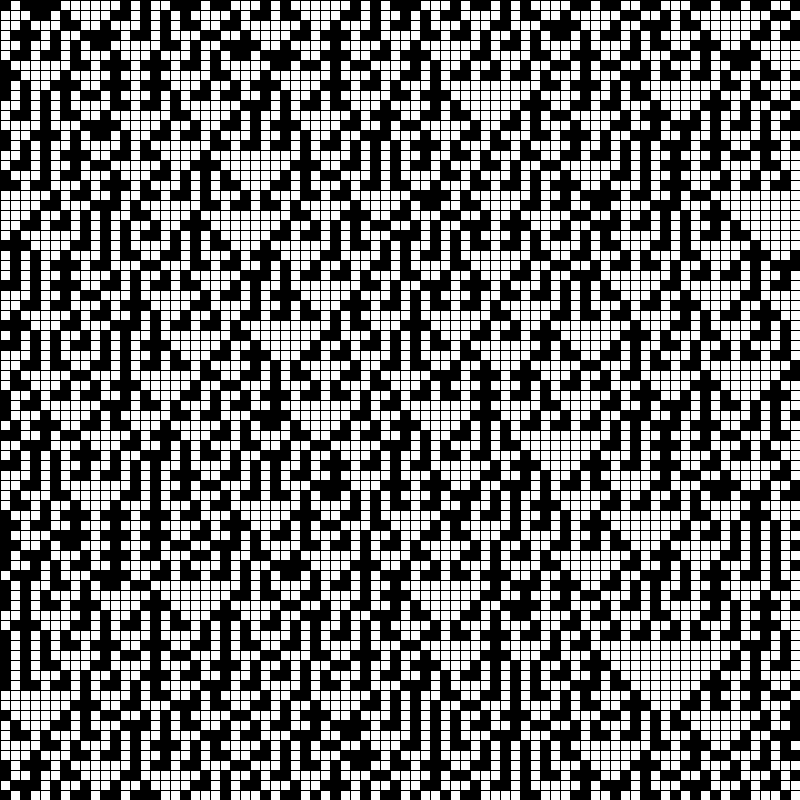
\includegraphics[width=0.17\textwidth]{figs/rule-150-best/rule-150-eval-15.png}}
		  &
		\fbox{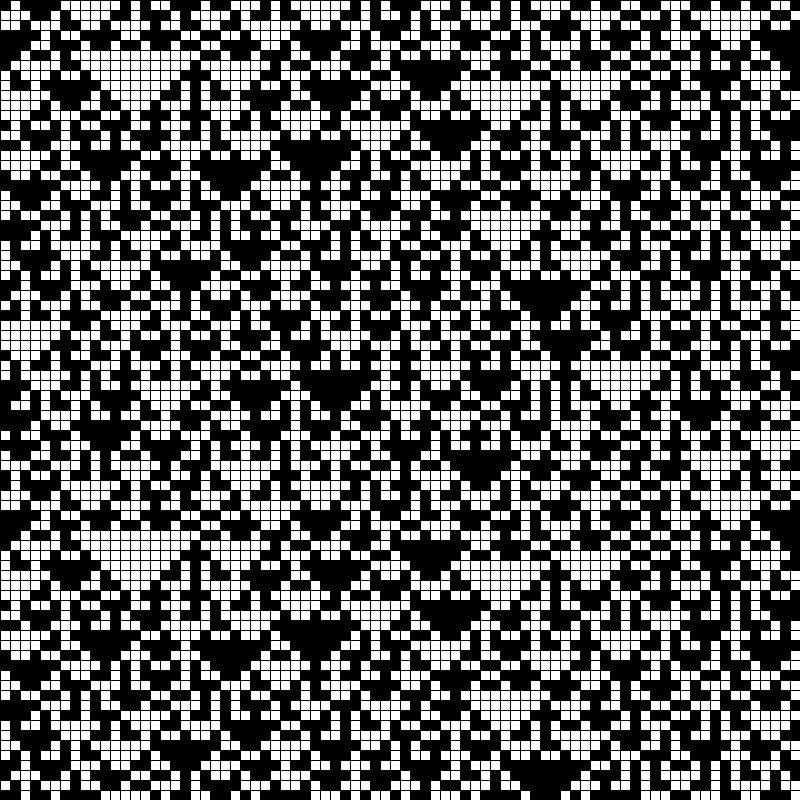
\includegraphics[width=0.17\textwidth]{figs/rule-150-best/rule-150-eval-16.png}} \\
		9 & 17 & 19 & 24 & 26                                                             \\
	\end{tabular}
	\caption{Current best individuals visualized with their space-time diagram and the corresponding GA iteration number, in R1.}\label{fig:best-150}
\end{figure*}

\begin{figure*}
	\centering
	\begin{tabular}{ccccc}
		\fbox{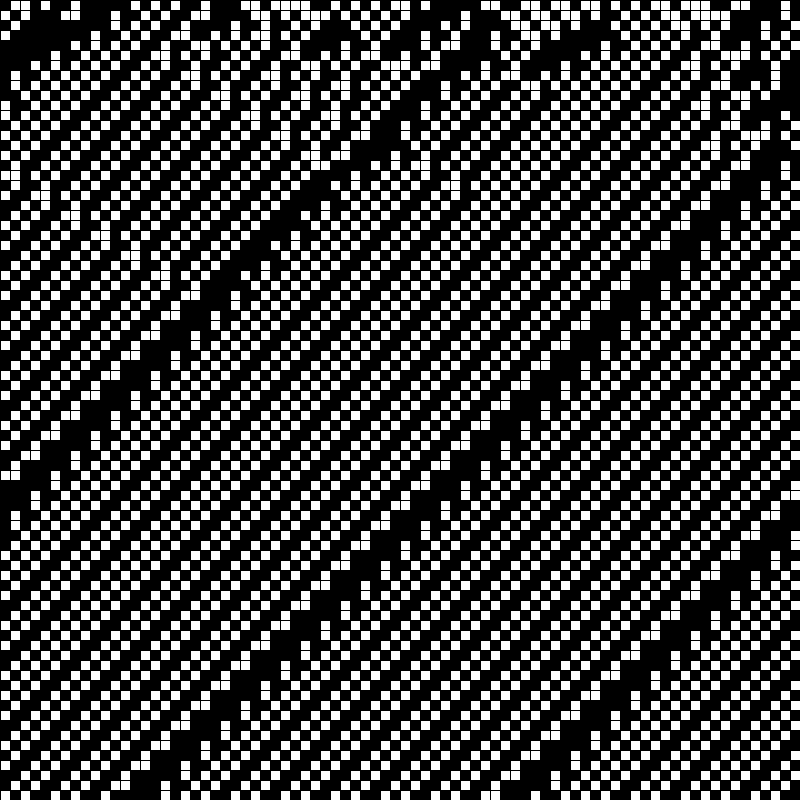
\includegraphics[width=0.17\textwidth]{figs/rule-184-best/rule-184-eval-1.png}}
		   &
		\fbox{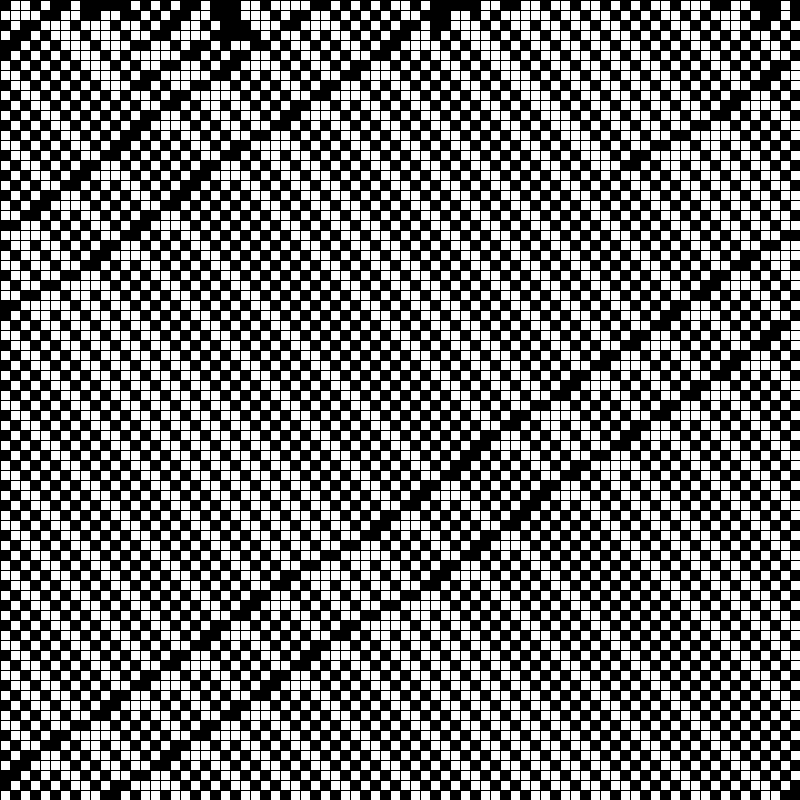
\includegraphics[width=0.17\textwidth]{figs/rule-184-best/rule-184-eval-2.png}}
		   &
		\fbox{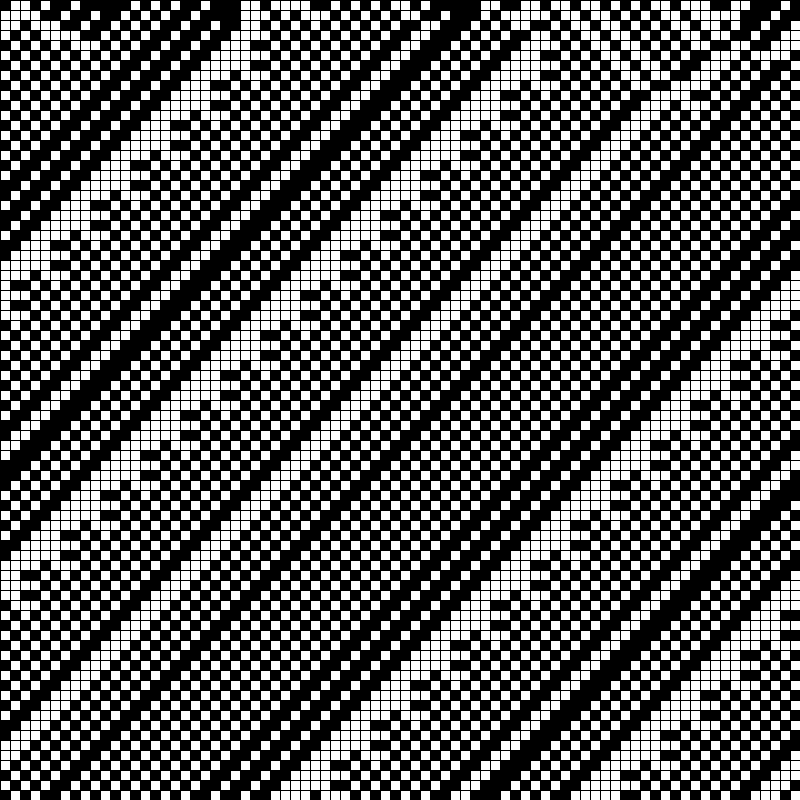
\includegraphics[width=0.17\textwidth]{figs/rule-184-best/rule-184-eval-3.png}}
		   &
		\fbox{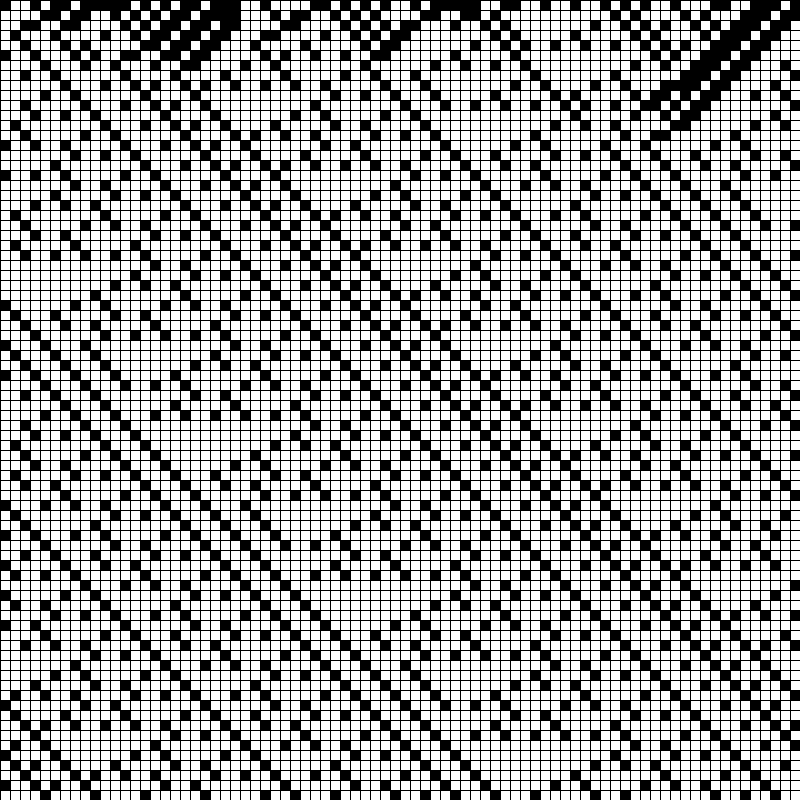
\includegraphics[width=0.17\textwidth]{figs/rule-184-best/rule-184-eval-4.png}}
		   &
		\fbox{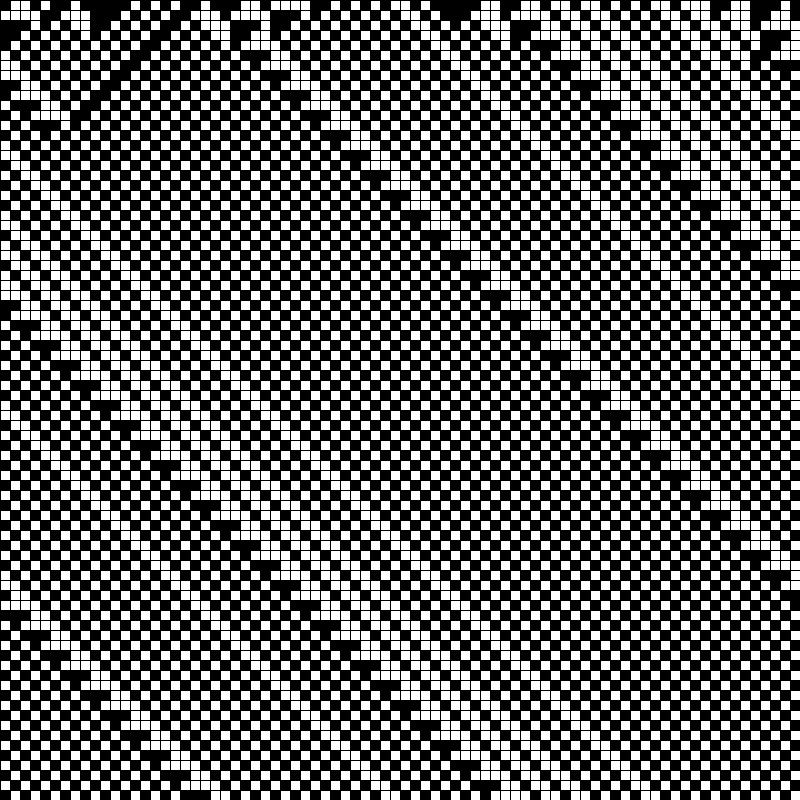
\includegraphics[width=0.17\textwidth]{figs/rule-184-best/rule-184-eval-5.png}}
		\\
		1  & 3  & 6  & 9  & 10 \\
		\fbox{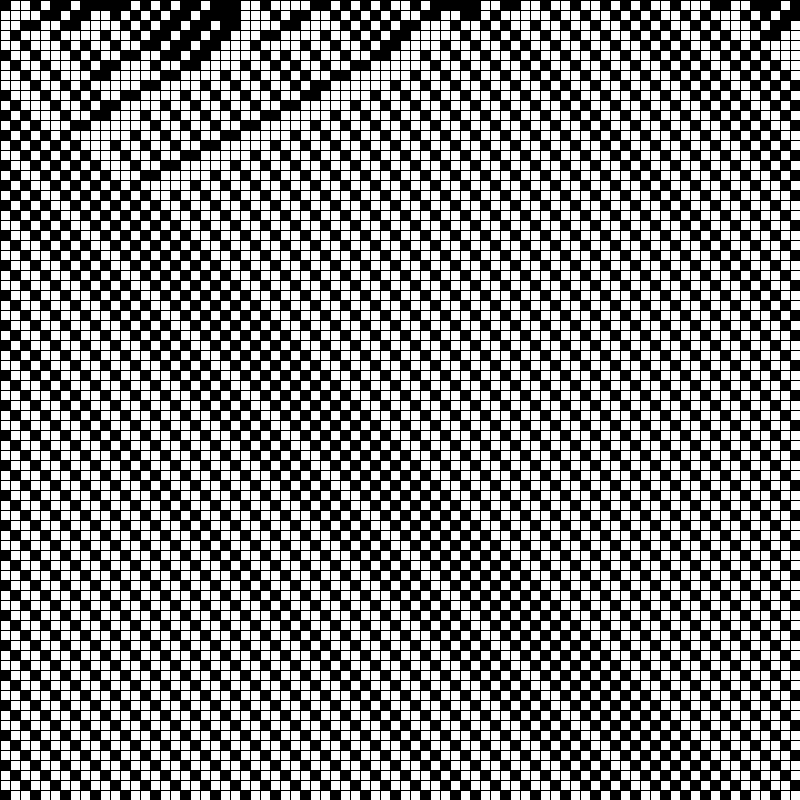
\includegraphics[width=0.17\textwidth]{figs/rule-184-best/rule-184-eval-6.png}}
		   &
		\fbox{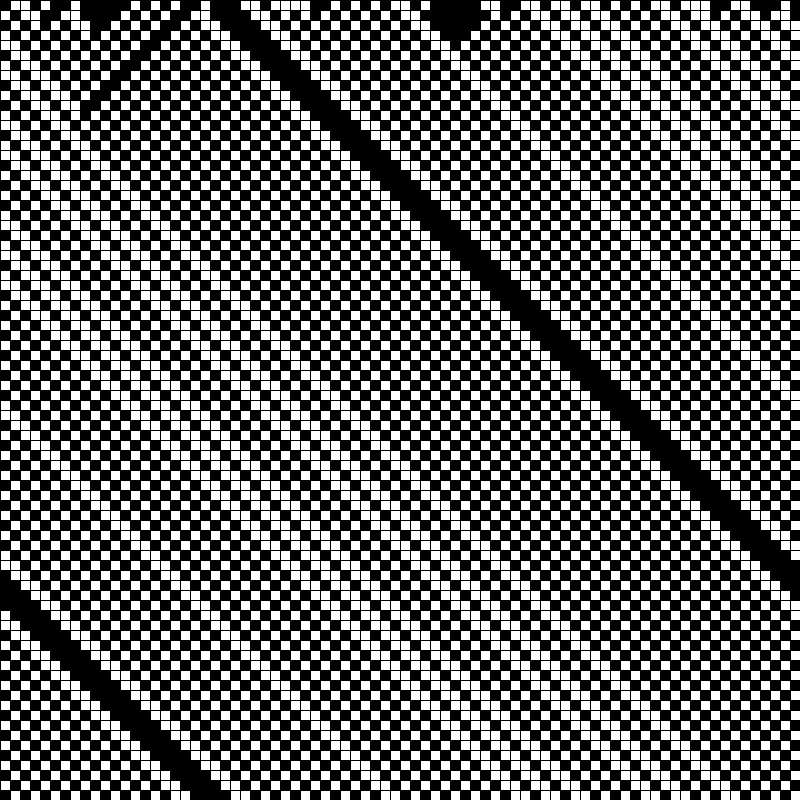
\includegraphics[width=0.17\textwidth]{figs/rule-184-best/rule-184-eval-7.png}}
		   &
		\fbox{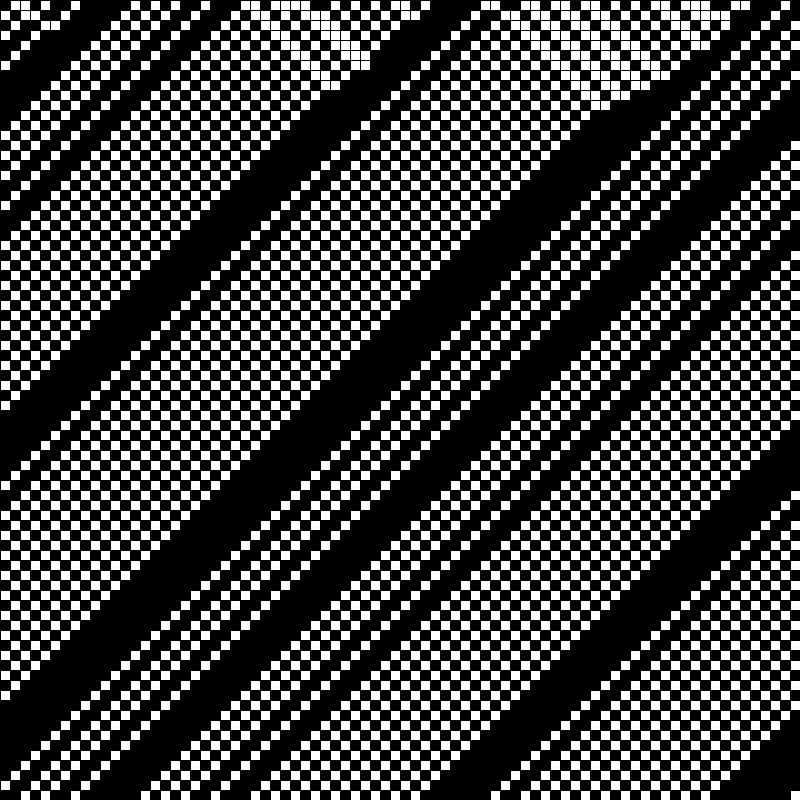
\includegraphics[width=0.17\textwidth]{figs/rule-184-best/rule-184-eval-8.png}}
		   &
		\fbox{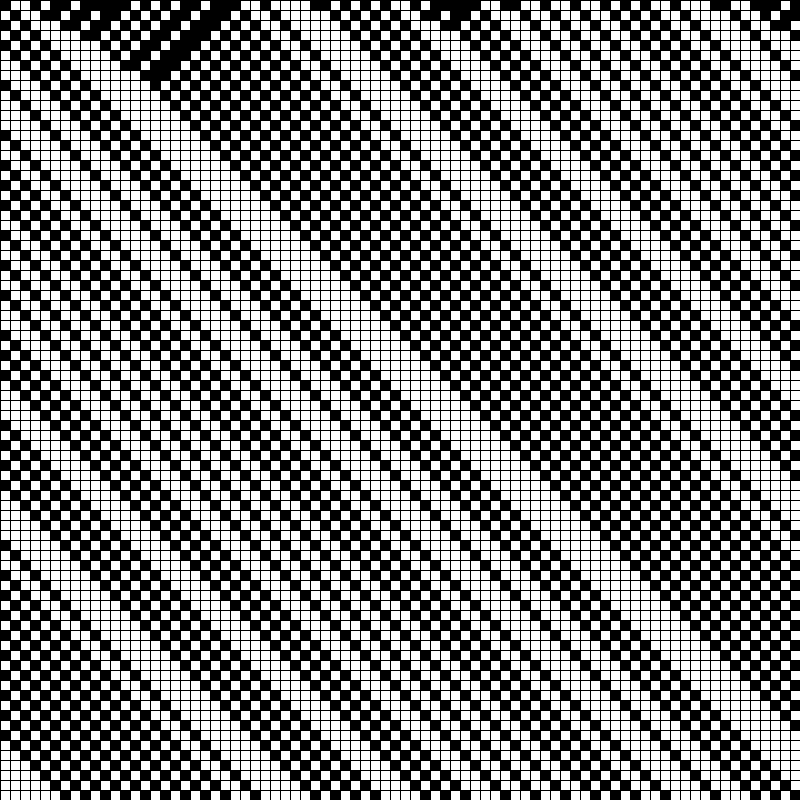
\includegraphics[width=0.17\textwidth]{figs/rule-184-best/rule-184-eval-9.png}}
		   &
		\fbox{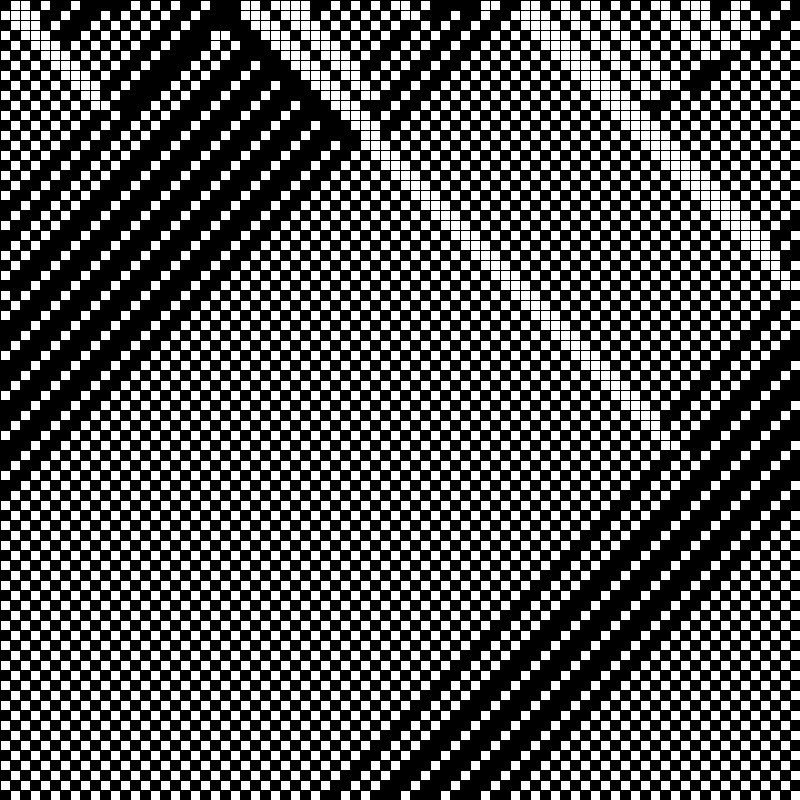
\includegraphics[width=0.17\textwidth]{figs/rule-184-best/rule-184-eval-11.png}}
		\\
		11 & 13 & 14 & 15 & 17 \\
		\fbox{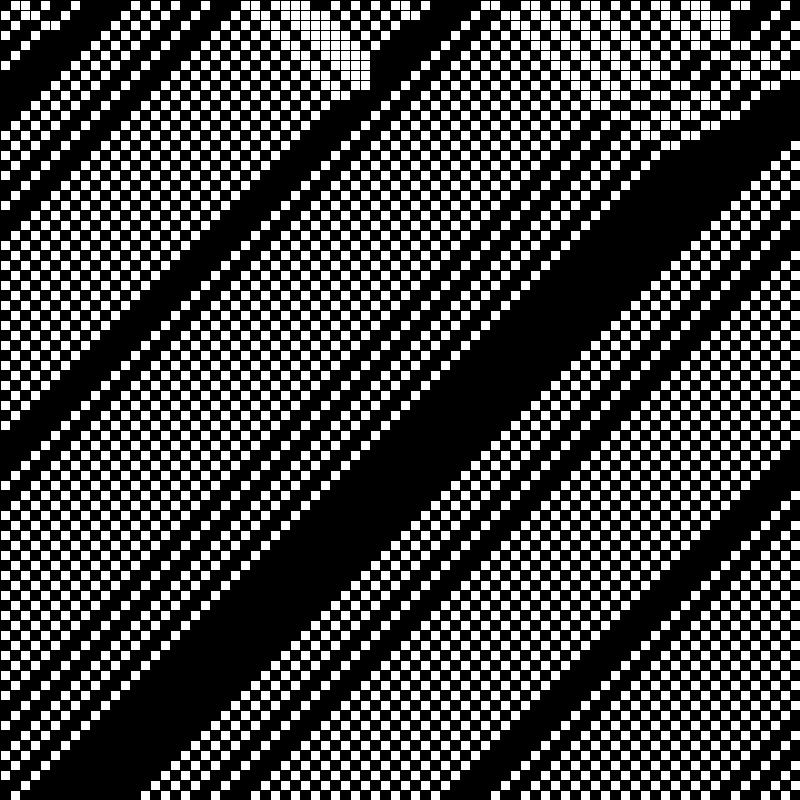
\includegraphics[width=0.17\textwidth]{figs/rule-184-best/rule-184-eval-12.png}}
		   &
		\fbox{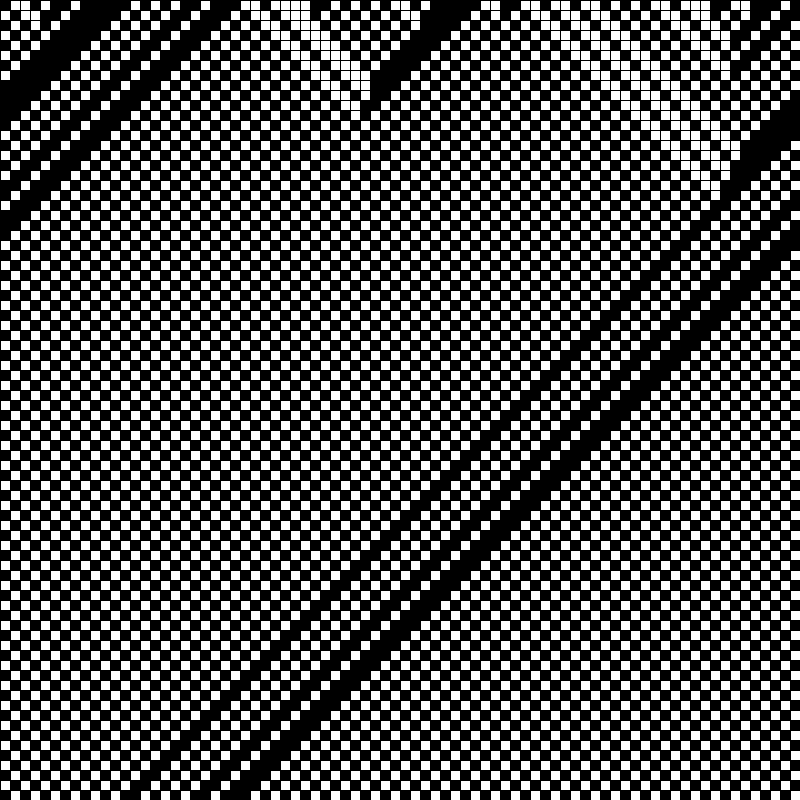
\includegraphics[width=0.17\textwidth]{figs/rule-184-best/rule-184-eval-13.png}}
		   &
		   &
		   &
		\\
		19 & 23 &    &    &
	\end{tabular}
	\caption{Current best individuals visualized with their space-time diagram and the corresponding GA iteration number, in R2.}\label{fig:best-184}
\end{figure*}

In Fig.~\ref{fig:best-150} we see the space-time diagram of some CAs that  were discovered by the GA during the evolution as ``current best'' candidates for R1, while Fig.~\ref{fig:best-184} displays these for R2.

Interestingly, in both experiments, relatively early in the evolution the GA was able to concentrate on some of the crucial patterns in the space-time diagrams of the unknown ECAs. In R1, after 6 iterations, the best individuals already replicated the triangular pattern of ECA 150, even though it is very hard to notice such a pattern in the observations available for the GA (see Fig.~\ref{fig:ob-eca150}). Similarly, in R2, the linear pattern emerged very quickly, yet deciding on the slope of the lines turned out to be a bit more challenging.